\chapter{L'approche items-to-skills mapping} 
\minitoc
\thispagestyle{empty}
\newpage
\section{Introduction}
Les systèmes éducatifs contiennent un grand nombre d'items (problèmes, questions). Ces éléments sont proposés aux apprenants à résoudre. Ceci est particulièrement vrai pour les systèmes adaptatifs, qui tentent de présenter des éléments adaptés à différents types d'apprenants. La gestion d’un grand nombre d’éléments est très difficile. Ainsi, les systèmes éducatifs collectent des données sur les performances des apprenants et ces données peuvent être utilisées pour obtenir un aperçu des propriétés des éléments. [1] \\
Dans ce chapitre, nous présentons les approches pour mapper les éléments aux compétences. En outre, nous décrivons les concepts de l'approche de similarité avec ses différentes catégories, et nous représentons les différentes mesures de similitude telles que Pearson, Kappa, Yule et Fisher.
\section{Knowledge (La connaissance)}
\subsection{Définition}
"Compréhension ou information sur un sujet que vous obtenez par expérience ou étude, soit connue par une personne ou par des personnes". [Dictionnaire Cambridge] La « connaissance » en éducation est constituée de faits de base alors que les composants de connaissance peuvent être des procédures, des schémas d'intégration, des stratégies de raisonnement complexes, des compétences métacognitives ..., c'est-à-dire (1er niveau de la taxonomie de Bloom (1956)). \\
La « connaissance » en philosophie est une « croyance vraie justifiée » alors que notre utilisation des éléments de connaissance comprend à la fois une connaissance incorrecte (fausse) et une connaissance implicite (sans croyance ou justification explicite). [2]

\subsection{Knowledge component (Composante connaissance)}
Un élément de connaissance est une description d'une structure mentale ou d'un processus qu'un apprenant utilise, seul ou en combinaison avec d'autres éléments de connaissance, pour accomplir les étapes d'une tâche ou d'un problème. (Koedinger, Corbett \& Perfetti, 2012) Les items qui requièrent la même compétence pour différents apprenants constituent une composante de connaissance (KC) [3]. \\
Composante de connaissance est un terme que nous utilisons tous les jours comme concept, principe, fait ou compétence, et des termes de sciences cognitives comme schéma, règle de production, idée fausse ou facette. [4]
La description de la composante de connaissance est présentée dans la figure \ref{knowledge_component}.

\begin{figure}[H]
	\begin{center}
		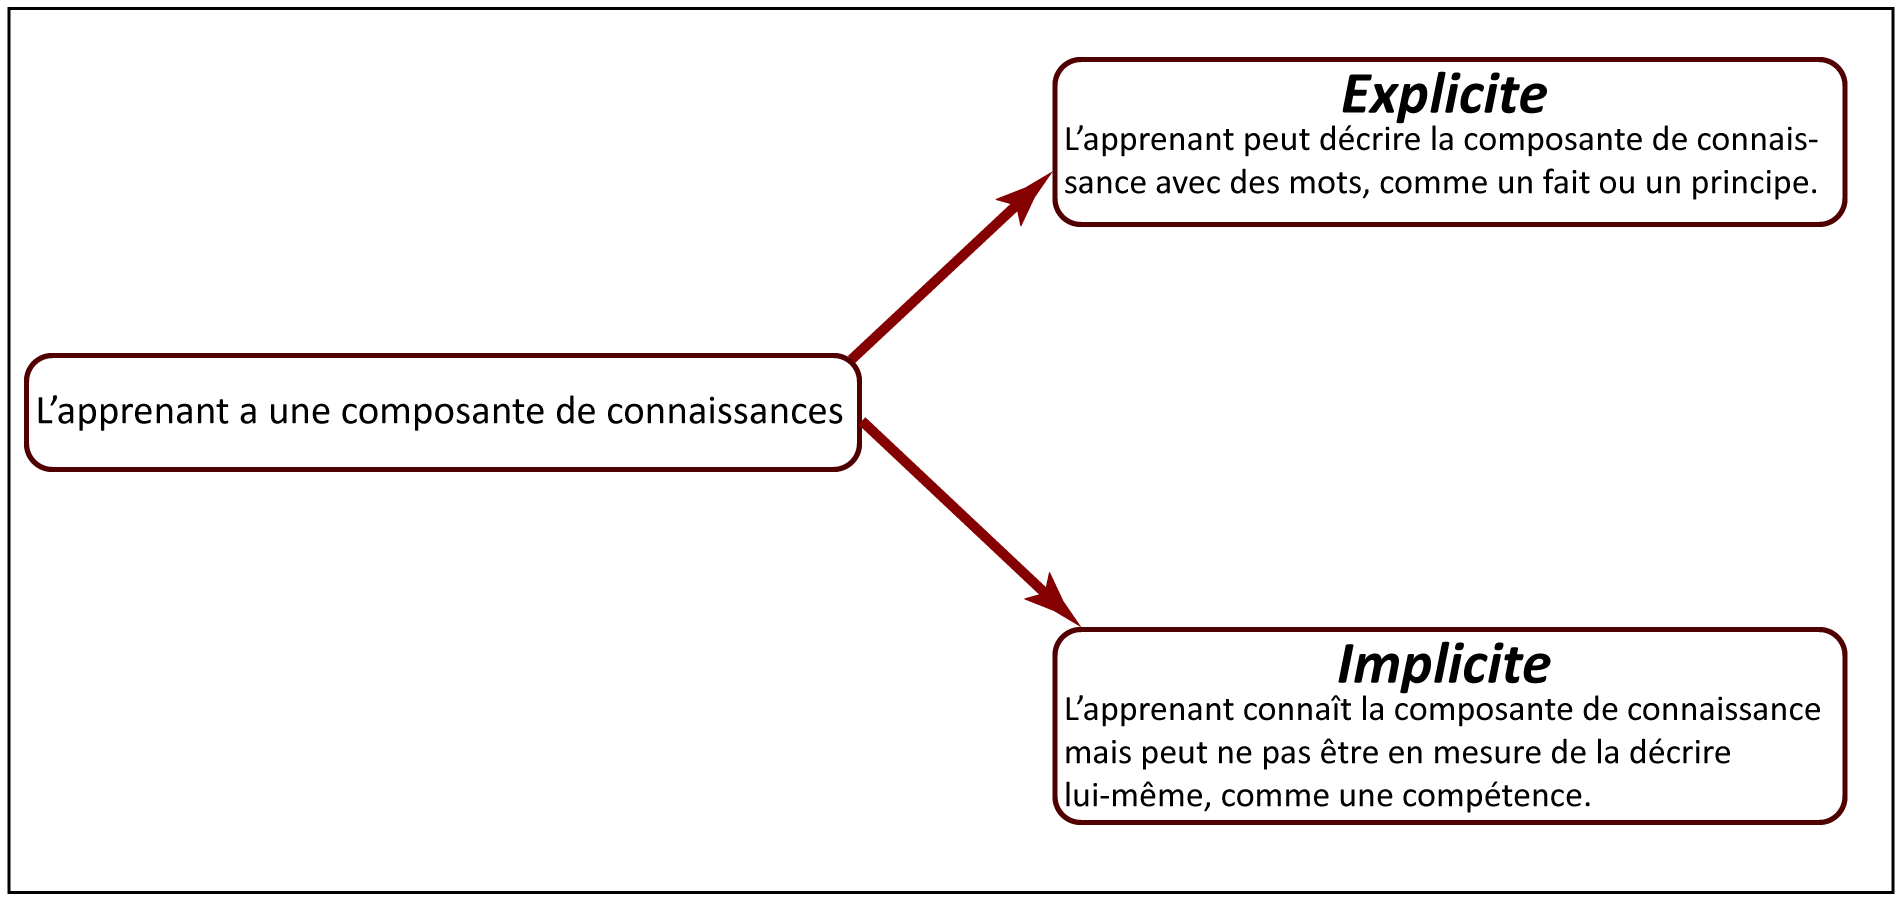
\includegraphics[width=\textwidth]{images/chapitre3/Knowledge_component.png}
	\end{center}
\caption{Knowledge Component}
\label{knowledge_component}
\end{figure}
\textbf{\underline{Exemple :}}
"Si l'angle A = 60 et (A = B, C = 60) Alors triangle équilatéral." \\
L'élève peut dessiner un triangle équilatéral sans être capable de décrire la règle. Une grande partie de ce que les apprenants de première langue savent de leur langue maternelle implique des éléments de connaissances implicites. Pertinence : la plupart des composants de connaissance explicites impliquent de nombreux composants de connaissance tacites (compétences innées ou acquises, le savoir-faire et l'expérience). La réponse et la fonctionnalité sont liées par la composante de connaissance, où les deux peuvent être externes, dans le monde, comme des signaux dans un stimulus et une réponse motrice ou interne, dans l'esprit, comme des fonctionnalités inférées et un nouvel objectif. [4].

\subsection{Les types de composante de connaissance}

La composante de connaissance est une représentation mentale de : [5]

\begin{itemize}
    \item[$\bullet$] \textbf{Connaissance du domaine :} faits, concepts, principes, règles, procédures, stratégies.
    \item[$\bullet$] \textbf{Connaissances préalables :} connaissance de l'encodage des fonctionnalités.
    \item[$\bullet$] \textbf{Connaissance intégrative :} schémas ou procédures qui connectent d'autres KC.
    \item[$\bullet$] \textbf{Connaissances métacognitives :} sur les connaissances, le contrôle de l'utilisation ou l'acquisition des connaissances.
    \item[$\bullet$] \textbf{Croyances et intérêts :} ce que l'on aime, croit.
    \item[$\bullet$] \textbf{Toute représentation externe des connaissances :} (comme les descriptions de manuels ou un exemple) ou les structures cognitives génériques (mémoire de travail), soit, les paramètres continus sur les représentations des connaissances (force, niveau d'engagement, valeur implicite d'un objectif, affect) ne sont pas des composants de connaissances.
\end{itemize}

\section{Items-to-skills mapping}
\subsection{Définition}
Mapper les éléments aux compétences latentes est l'automatisation de la découverte des compétences derrière les éléments de question à des fins d'ingénierie cognitive est hors de portée dans l'état actuel de la recherche, des moyens pour aider à déterminer le nombre de compétences et les compétences communes entre les éléments est un effort raisonnable au milieu -terme. [6]

\subsection{items-to-skills mapping Structure}
Il existe deux approches de la cartographie des éléments aux compétences présentées dans la figure \ref{items_to_skills_mapping}:

\begin{figure}[H]
	\begin{center}
		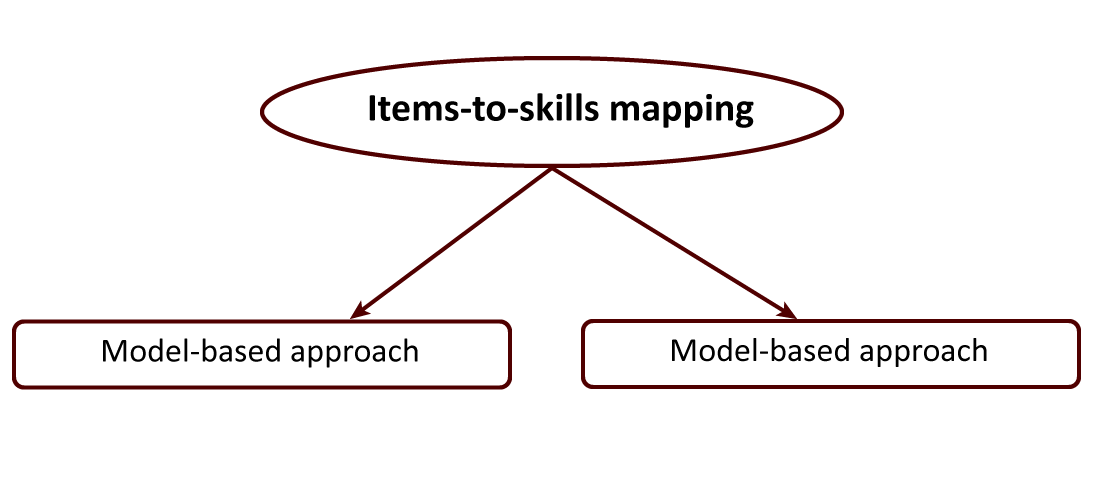
\includegraphics[width=\textwidth]{images/chapitre3/Items_to_skills_mappin_structure.png}
	\end{center}
\caption{Items-to-skills mapping Structure}
\label{items_to_skills_mapping}
\end{figure}

\subsubsection{Model-Based approach}
\paragraph{Définition}
La construction d'un modèle simplifié qui explique les données observées. Basé sur une matrice de réponses des apprenants aux éléments, le modèle prédit les réponses de l'apprenant. Le modèle attribue plusieurs compétences latentes aux apprenants et utilise une cartographie des éléments aux facteurs latents correspondants. Ce type de modèle peut souvent être exprimé naturellement à l'aide de la multiplication matricielle, c'est-à-dire que l'ajustement d'un modèle conduit à une factorisation matricielle. Une fois que nous obtenons le résultat après avoir ajusté le modèle aux données, nous avons désigné les items avec la même valeur d'un facteur latent comme « similaires ». Cette approche conduit naturellement à plusieurs composantes de connaissance par compétence. [1] Le modèle basé sur le modèle présenté dans la figure \ref{model_based} développe un modèle de notation des utilisateurs, les algorithmes de cette catégorie adoptent une approche probabiliste en calculant la valeur attendue de la prédiction de l'utilisateur et en tenant compte des notes de l'utilisateur sur d'autres éléments. [8] \\
Le processus de modèle peut être produit par différents algorithmes d'apprentissage automatique tels que le réseau bayésien, le clustering et l'approche basée sur des règles. [7]

\begin{figure}[H]
	\begin{center}
		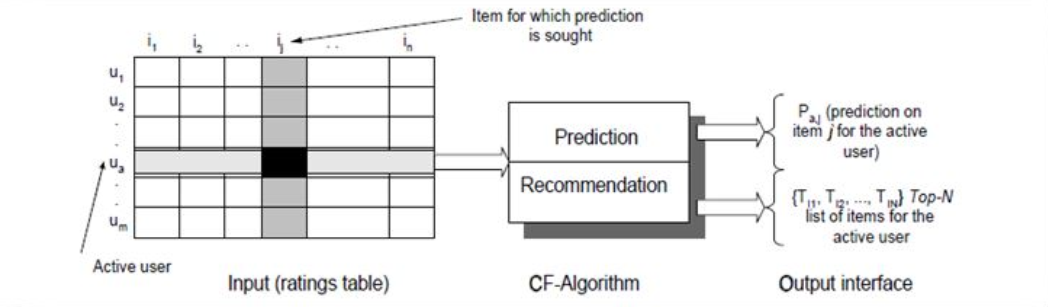
\includegraphics[width=\textwidth]{images/chapitre3/Model_based.png}
	\end{center}
\caption{Model based}
\label{model_based}
\end{figure}

Cette approche guide des composants de connaissances différents et multiples par compétence. Le modèle est généralement calculé à l'aide d'une technique d'optimisation qui ne mène qu'à des optima locaux (par exemple, une descente de gradient). \\
Dans les systèmes recommandés, cette approche est utilisée pour la mise en œuvre du filtrage collaboratif ; elle est souvent appelée "Décomposition en valeurs singulières" (SVD). [9] 

\paragraph{Model Based Techniques}
Dans le contexte pédagogique, de nombreuses variantes de l'approche basée sur les modèles ont été proposées : \\

\begin{itemize}
    \item[$\bullet$] \textbf{Q-matrix :} Est une matrice binaire illustrée à la figure 4 montrant la relation entre les éléments de test et les attributs ou concepts latents ou sous-jacents (Birenbaum, et al., 1993). Les états de connaissance ont été attribués aux apprenants en fonction de leurs réponses aux tests et de la matrice q construite. [10]
\end{itemize}

\begin{figure}[H]
	\begin{center}
		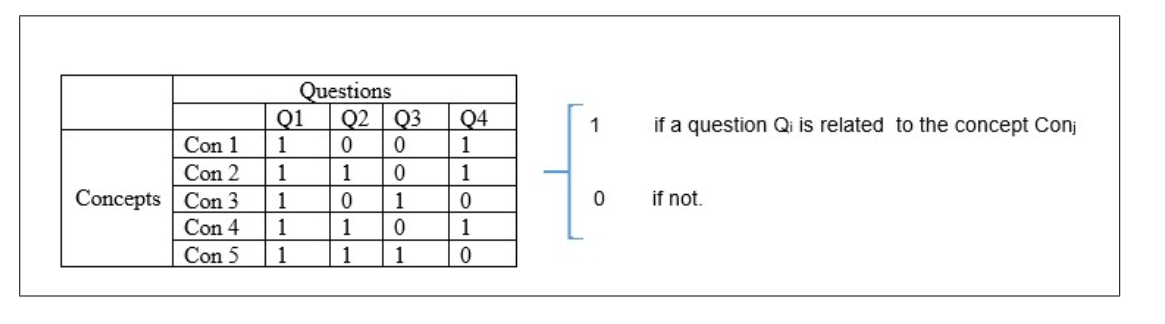
\includegraphics[width=\textwidth]{images/chapitre3/q_matrix.png}
	\end{center}
\caption{Q-matrix}
\label{q_matrix}
\end{figure}

\subsection{Similarity-based approach (Item-Similarity)}
\subsubsection{Définition}
En statistiques et en mathématiques, la mesure de similarité ou la fonction de similarité est une fonction à valeur réelle qui mesure la similarité entre deux éléments. Les valeurs de similarité entre les éléments sont quantifiées par l'observation de la performance des utilisateurs sur les éléments, qu'il s'agisse de négatif ou non [11]. La mesure des similitudes est une étape très importante dans une analyse plus approfondie telle que le regroupement des éléments, ce qui est utile à plusieurs égards. [12]  \\
Dans cette approche, nous calculons directement une mesure de similarité pour chaque paire d'éléments. Ces similitudes sont ensuite utilisées pour faire le clustering, pour faire la visualisation en projetant ces éléments dans un plan a 2 ou 3 dimensions, ou pour faire d’autre analyse en essayant de récupérer les éléments les plus similaire. Cette approche est illustrée à la figure \ref{illustration_item_similarity}. 

\begin{figure}[H]
	\begin{center}
		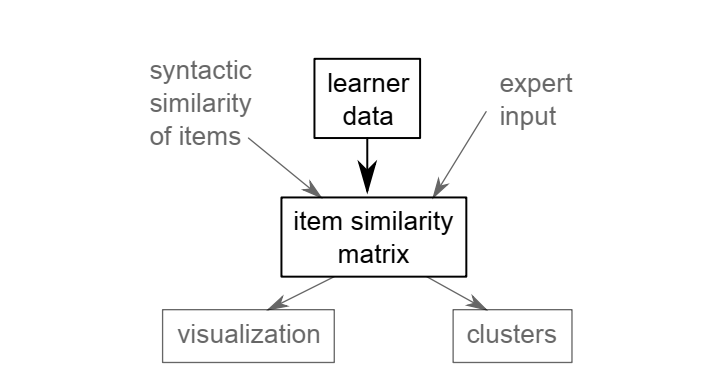
\includegraphics[width=\textwidth]{images/chapitre3/Illustration_item_smilarity.png}
	\end{center}
\caption{Illustration de l'approche générale de l'analyse des éléments basée sur les similitudes des éléments.}
\label{illustration_item_similarity}
\end{figure}

Dans l'apprentissage éducatif, la définition de la similarité des éléments a été analysée en utilisant la corrélation des réponses des apprenants et les temps de résolution des problèmes, ainsi qu'en utilisant les mauvaises réponses des apprenants. [12]

\subsubsection{Processus de similarité des items (éléments)}
Une étape importante de l'approche basée sur les items consiste à calculer le degré de similitude entre chaque paire d’items, puis à sélectionner les éléments les plus similaires. Il peut être décrit comme l'opération de calcul de similarité entre deux éléments i et j, où il s'agit d'abord de définir les utilisateurs qui ont évalué ces deux éléments, puis d'appliquer une technique de calcul de similarité pour déterminer le score de similarité entre i et j. [13] La figure \ref{calcul_application_similarity} ci-dessous montre l'approche générale du calcul et de l'application de la similarité des items.

\begin{figure}[H]
	\begin{center}
		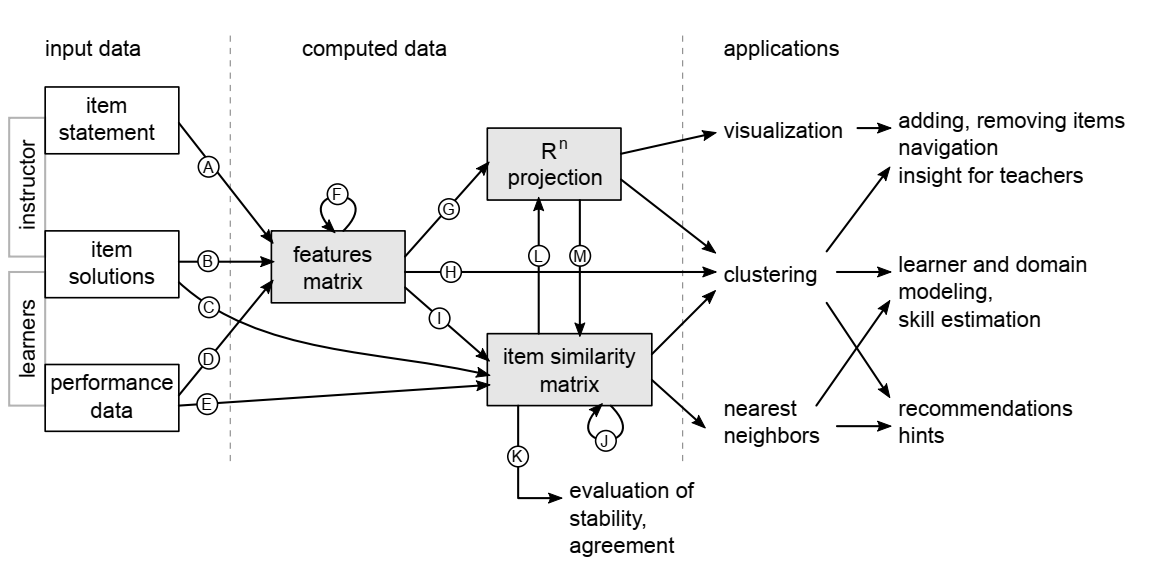
\includegraphics[width=\textwidth]{images/chapitre3/calcul_application_similarity.png}
	\end{center}
\caption{L'approche générale du calcul et de l'application de la similarité des éléments.}
\label{calcul_application_similarity}
\end{figure}

Nous allons brièvement parcourir les trois étapes input data, computed data, applications illustrées dans la figure \ref{calcul_application_similarity}. 
\paragraph{Input Data}

\begin{itemize}
    \item \underline{Item statement (Arrow A) :} Un énoncé d'item dans est la spécification de la tâche que l'apprenant doit résoudre donnée en langage naturel, ou des exemples d'entrée-sortie.
    
    \begin{itemize}
		\item La construction de la matrice des fonctionnalités nécessite d'abord un prétraitement à l'item qu'il soit en langage naturel,
		\item Les techniques du modèle du sac de mots qui permettent par exemple de représenter le texte par un vecteur avec le nombre d'occurrences de chaque mot
		\item D'autres caractéristiques peuvent être obtenues à partir de la spécification des données d'entrée, par exemple, les types de variables (entier, chaîne, liste)
	\end{itemize}
	
\end{itemize}

\begin{itemize}
    \item \underline{Item solution} Est simplement la solution donnée par l’apprenant ou la solution commune des apprenants. Elle est présentée comme un programme dans un langage de programmation donné.
    
    \begin{itemize}
		\item Feature Matrix : (Arrow B)
		\begin{itemize}
			\item Analyse du code source jusqu'aux fonctions de calcul décrivant l'apparition des concepts de programmation et des mots-clés (alors, if, return,print, ) soit l'utilisation d'opérateurs.
			\item Le modèle du sac de mots est appliqué uniquement sur les mots-clés de programmation au lieu de mots dans un langage naturel.
		\end{itemize}

		\item Direct computation of similarities: (Arrow C)
		\begin{itemize}
			\item Le calcul de la distance entre les solutions choisies des deux items.
			\item Il est calculé par plusieurs méthodes, par exemple : distance d'édition d'arbre d'exemple pour l'arbre de syntaxe abstraite, ou la distance d'édition de base de Levenshtein pour le code canonisé.
		\end{itemize}
	\end{itemize}
	
\end{itemize}

\begin{itemize}
    \item \underline{Performance data} Informations sur la performance des apprenants lors de la résolution des items par exemple : exactitude de la réponse, temps de réponse, nombre d'indices utilisés et nombre de tentative faite sur un seul item.
    
    \begin{itemize}
		\item Feature matrix (Arrow D) : Les données sont transformées en fonctionnalités telles qu'un écart de performance ou le ratio d'apprenants qui ont résolu l'élément correctement.

		\item Direct computation of similarities: (Arrow E)
		\begin{itemize}
			\item La similitude des items i, j est le résultat du calcul de leur corrélation basé sur les performances des apprenants qui ont résolu les items i et j.
			\item Il peut être calculé en utilisant la méthode de correction (réponse correcte/incorrecte) ou la méthode des temps de résolution (plutôt que la correction).
		\end{itemize}
	\end{itemize}
	
\end{itemize}

\paragraph{Computed Data}

\begin{itemize}
    \item \underline{Features matrix :} c'est la matrice qui contient les éléments et leurs caractéristiques qui peuvent être par exemple une solution d'élément ou des mots-clés apparaissant dans une déclaration d'élément. La matrice de caractéristiques peut être normalisée ou transformée (flèche F) à l'aide de techniques telles que la transformation terme fréquence-fréquence inverse du document. La matrice de caractéristiques peut être normalisée ou transformée (flèche F) à l'aide de techniques telles que la transformation terme fréquence-fréquence inverse du document.A partir de la matrice de caractéristiques, nous pouvons calculer une projection sur Rn (flèche G et flèche L). La projection est généralement utilisée pour des applications, en particulier pour la visualisation d'éléments. Cependant, cela peut également être une étape de traitement utile dans le calcul des similitudes d'articles, par exemple, pour décorréler des caractéristiques.
	\item \underline{Item similarity matrix :} est une matrice bidimensionnelle m, où m[i,j] désigne la similarité des items i et j. Le calcul de la matrice de similarité basée sur la matrice de caractéristiques (flèche I) ou sa projection dans Rn (flèche M) est une opération courante en apprentissage automatique, avec de nombreux choix disponibles, par exemple la similarité cosinus, le coefficient de corrélation de Pearson et la distance euclidienne (transformé en mesure de similarité par soustraction).
\end{itemize}

\subsubsection{Item-Similarity measures}
Pour calculer le score de similarité entres deux items, il faut tout d’abord créer la matrice d’accord entre item i et item j. Cette matrice d’accord appeler aussi matrice de confusion ou (confusion matrix en anglais) est illustrer par le tableau 3.

\begin{table}[!htbp]
    \centering
	\begin{tabular}{|c| c|c|}
	\hline
	 & Item i (Correct) & Item i (Incorrect)  \\ \hline
	 Item j (Correct) & a & b  \\  \hline
	 Item j (Incorrect) & c & d  \\  \hline
	\end{tabular}
	\caption{La matrice d’accord pour deux items}
	\label{matrice_accord}
\end{table}

Ensuite cette matrice d’accord est utilisée pour calculer la similarité entre l’item i et j. Les coefficients de calcule de similarité qui peuvent être utiliser sont les suivants (Figure 4) :

\begin{table}[!htbp]
    \centering
	\begin{tabular}{|c| c|}
	\hline
	Mesures & Equation  \\ \hline
	Yule  & \(\displaystyle Sy = (ad-bc)/(ad+bc)\)   \\  \hline
	Pearson  &  \(\displaystyle Sp = (ad-bc)/\sqrt{(a+b)(a+c)(b+d)(c+d)}\) \\ \hline
	\makecell{\\Cohen \\ \\ \\}  & \makecell{\(\displaystyle Sc = (Po-Pe)/(1-Pe) \) \\ \(\displaystyle Po = (a+d)/n\) \\  \(\displaystyle Pe = ((a+b)(a+c)+(b+d)(c+d))/n^{2} \)}  \\  \hline
	Sokal  & \(\displaystyle Ss = (a+b)/(a +b +c + d)  \)   \\  \hline
	Jaccard  & \(\displaystyle Sj = a/(a+b+c) \)   \\  \hline
	Ochiai  & \(\displaystyle So = a/\sqrt{(a+b)(a+c)} \)   \\  \hline
	\end{tabular}
	\caption{Ccv}
	\label{differentes_mesures_similarité}
\end{table}

\section{Conclusion} 
Dans ce chapitre nous avons a introduit les concepts de base de la composante connaissance, la cartographie des approches des compétences, en spécifiant différentes similitudes qui peuvent ensuite être utilisées dans une analyse plus approfondie des relations d'un élément, telles qu'un regroupement d'éléments ou une visualisation. Ensuite, la revue de la littérature et les travaux connexes dans le domaine de l'apprentissage profond et de l'exploration de données éducatives.